\documentclass[pdf]{beamer}
\mode<presentation>{}

\usetheme{metropolis}
 
\usepackage{ulem}
\usepackage[francais]{babel}
\usepackage[utf8]{inputenc}
\usepackage[T1]{fontenc}
\usepackage{amsmath}
\usepackage{listings}
\usepackage{multimedia}
\usepackage{url}

\newcommand\gr{\selectlanguage{greek}}
\newcommand\fr{\selectlanguage{francais}}

\addtobeamertemplate{footline}{\insertframenumber/\inserttotalframenumber}

%% preamble

\title{Fouine 3.0}
\subtitle{Elles sont dans nos campagnes, dans nos villes... Elles sont sur les réseaux sociaux... }
\author{Bethune Louis, Felderhoff Joël}

%%document

\begin{document}

\begin{frame}
\titlepage
\end{frame}

\begin{frame}{Le parsing}
\begin{figure}
\center
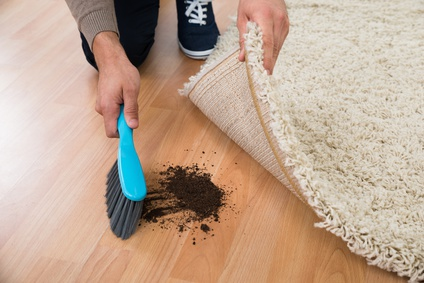
\includegraphics[scale=0.7]{les-petits-tas-de-poussiere-sous-nos-tapis.jpg} 
\caption {LA bonne réaction face aux shift-reduce}
\end{figure}
\end{frame}


\begin{frame}{La récursivité}
\begin{figure}
\center
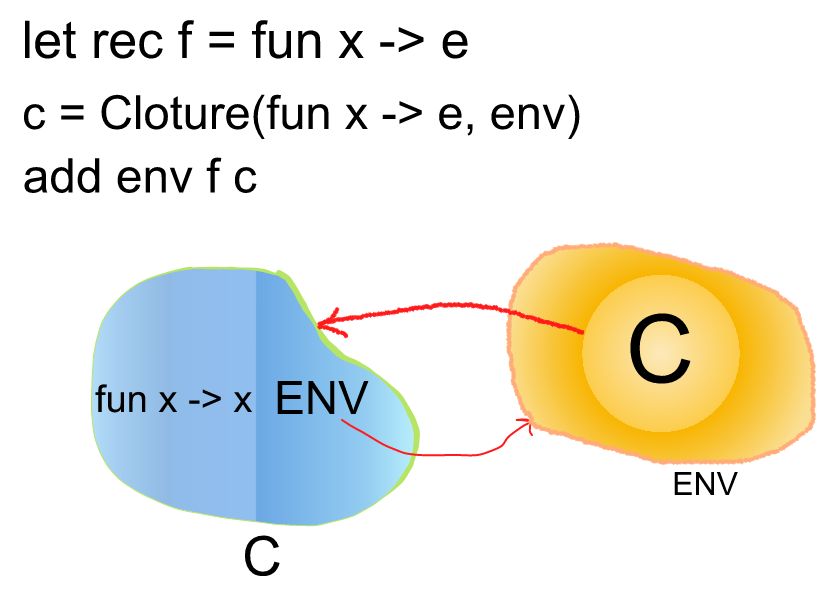
\includegraphics[scale=0.3]{Drawing.png} 
\caption {Phagocytose d'une clôture par une table de hachage}
\end{figure}
\end{frame}

\begin{frame}{Gestion des conflits }
Comment gérer les conflits (non, pas les shift/reduce) avec votre partenaire de Projet2 ?
\pause
\begin{itemize}
\item Vous avez tort
\pause
\item Votre binôme a raison
\pause
\item D'ailleurs c'est lui qui fait tout le travail
\pause
\item Le seul code que vous produisez est un simple nid de bug
\pause
\item Ce sont ses idées qui marchent, cherchez pas plus loin
\end{itemize}
\pause
Avec ça, vous êtes sûr que ça se passe bien
\pause

Évidemment, ça ne s'est PAS passé comme ça pour nous
\end{frame}

\begin{frame}{Gérer un partenaire chiant}
Comme on ne peut pas toujours appliquer les conseils de la slide précédente, comment faire pour gérer \sout{l'autre con} le binôme.

\pause

Cas concret : réponses du binôme à une question technique

\pause
\begin{center}
\vspace{-0.5cm}
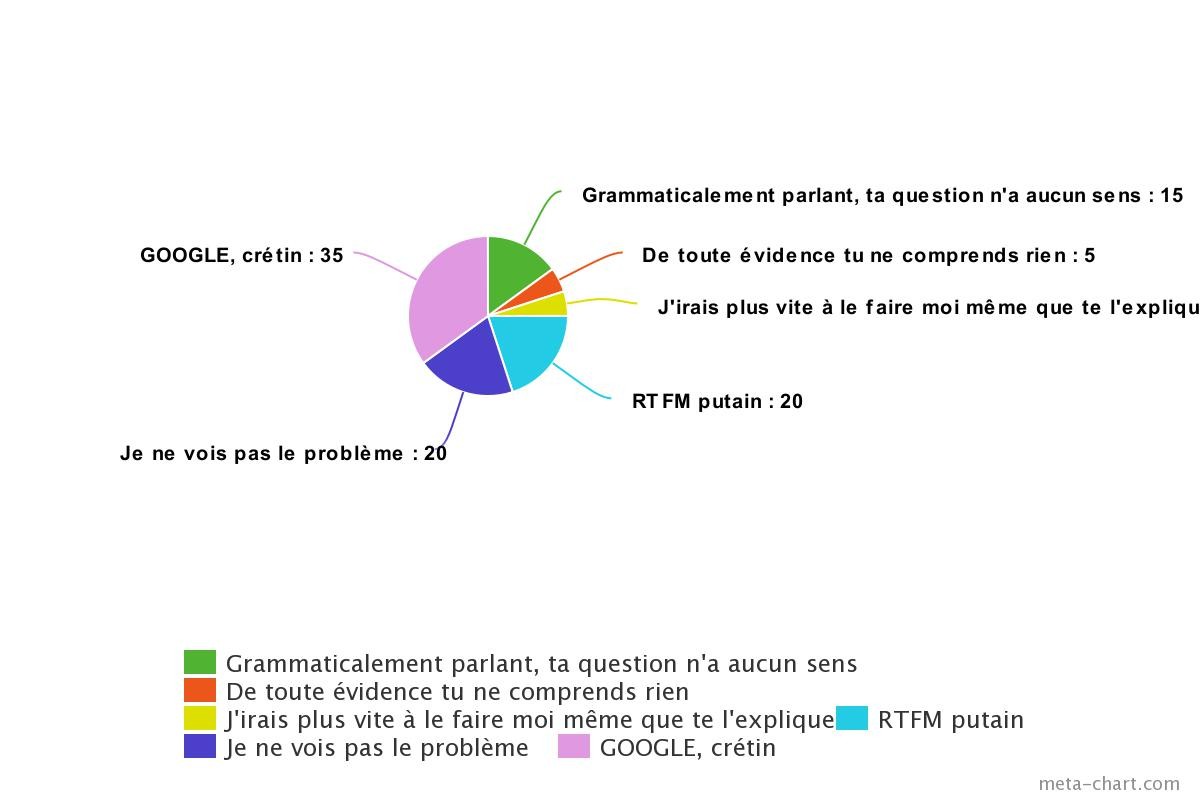
\includegraphics[scale=.24]{meta-chart}

\end{center}

\end{frame}

\begin{frame}{Conclusion}
Que faire dans ce cas là ? 
\pause

De toute façon il est 2h30 du matin, on commit, on push et tant pis
\end{frame}

\begin{frame}{Questions?}
Merci pour votre attention
\end{frame}

\end{document}

